	
	\appendixtitleon
	\appendixtitletocon
	\begin{appendices}

	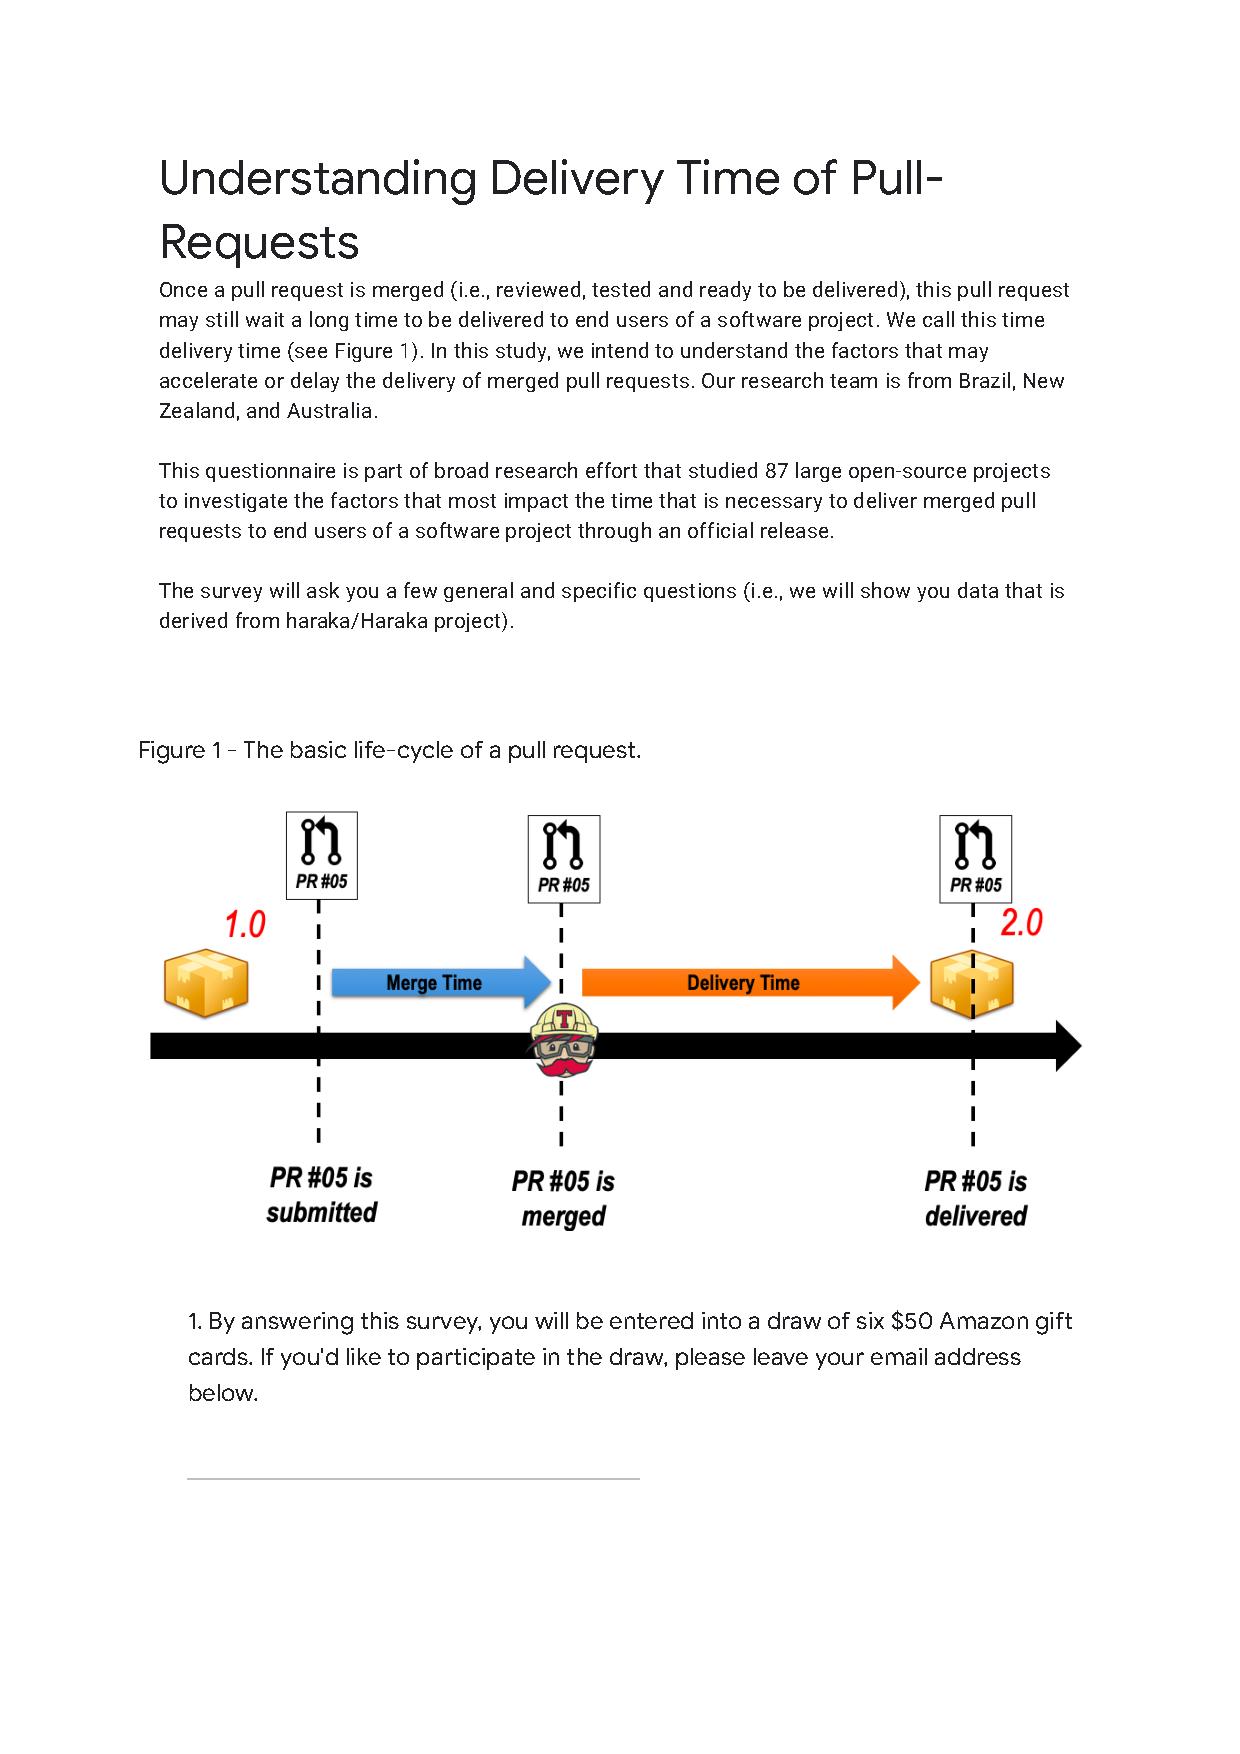
\includepdf[pages=1, width=\textwidth, 
	offset=-2cm 0cm,
	pagecommand=\section{Project Survey Example}
	\label{sec:appendix_project_survey_example}]{haraka_Haraka_form.pdf}	
		
	\includepdf[pages={2-11}, offset=2cm 2cm, width=12cm,
		offset=-2cm 0cm]
		{haraka_Haraka_form.pdf}	
	
	\section{Invitation Letter}
	\label{sec:appendix_invitation_latter}
	
	{\fontfamily{lmss}\selectfont

	\noindent
	MAIL SUBJECT: \textbf{Why do PRs take so long to be delivered? Research survey}
	\vspace{0.3cm} 
	
	\noindent
	Dear \textbf{\${contributor.name}},	
	\vspace{0.3cm} 

	\noindent
	We are a group of researchers from universities based in Brazil, Australia, and New Zealand. We are studying the impact of Continuous Integration on the time to release merged pull requests to end users of open source projects.
	\vspace{0.3cm} 
	
	\noindent
	We have collected public data from the project \textbf{\${project.fullName}} in the period from 
	
	\noindent
	\textbf{\${project.creationDate}} to 2016-11-11. According to our data, you have contributed \textbf{\${contributor.deliveredPRsCount}} pull-requests to \textbf{\${project.fullName}} which were effectively merged and delivered to end users. 
	\vspace{0.3cm} 
	
	\noindent
	As you were a contributor of the project \textbf{\${project.fullName}}, we would appreciate if you shared your experience with us by answering a few questions in the following survey: 
	\vspace{0.3cm} 
	
	\noindent
	Google Form: \textcolor{blue}{Understanding Delivery Time of Pull Requests}
	\vspace{0.3cm} 
	
	\noindent
	The survey has 24 questions (all of them are optional) and will take less than 15 minutes to complete. To compensate you for your time, all participants that answer all questions will be entered into a draw of six \$50 Amazon gift cards.
	\vspace{0.3cm} 
	
	\noindent
	Best Regards,
	\vspace{0.3cm} 
	
	\noindent
	Jo\~{a}o Helis Bernardo.
	
	\noindent
	PhD student at the Federal University of Rio Grande do Norte, Brazil.		
	}
	\newpage
	
	\section{Number of participants per project}
	\label{sec:appendix_participants_ids_and_their_projects}
	
	The number of participants per project are distributed in Tables \ref{tab:participants_per_project_part_i} and \ref{tab:participants_per_project_part_ii}.

	\begin{table*}[htb]
	\centering
	\caption{Number of participants per project and their IDs (PART I)}
	\begin{tabular}{|c|c|c|c|}
		\hline
		\textbf{\#} & \multicolumn{1}{c|}{\textbf{project}} & \textbf{participants IDs } & \textbf{total of participants} \bigstrut\\
		\hline
		1     & grails/grails-core & C001 -- C005 & 5 \bigstrut\\
		\hline
		2     & saltstack/salt & C006 -- C035 & 30 \bigstrut\\
		\hline
		3     & mozilla-b2g/gaia & C036 -- C042 & 7 \bigstrut\\
		\hline
		4     & rails/rails & C043 -- C066 & 24 \bigstrut\\
		\hline
		5     & owncloud/core & C067 -- C079 & 13 \bigstrut\\
		\hline
		6     & cakephp/cakephp & C080 -- C092 & 13 \bigstrut\\
		\hline
		7     & ipython/ipython & C093 -- C097 & 5 \bigstrut\\
		\hline
		8     & ansible/ansible & C098 -- C113 & 16 \bigstrut\\
		\hline
		9     & fog/fog & C114 -- C125 & 12 \bigstrut\\
		\hline
		10    & appcelerator/titanium\_mobile & C126  & 1 \bigstrut\\
		\hline
		11    & TryGhost/Ghost & C127 -- C133 & 7 \bigstrut\\
		\hline
		12    & mozilla/pdf.js & C134 -- C139 & 6 \bigstrut\\
		\hline
		13    & elastic/kibana & C140 -- C143 & 4 \bigstrut\\
		\hline
		14    & AnalyticalGraphicsInc/cesium & C144 -- C147 & 4 \bigstrut\\
		\hline
		15    & twbs/bootstrap & C148 -- C150 & 3 \bigstrut\\
		\hline
		16    & sympy/sympy & C151 -- C157 & 7 \bigstrut\\
		\hline
		17    & matplotlib/matplotlib & C158 -- C169 & 12 \bigstrut\\
		\hline
		18    & scipy/scipy & C170 -- C185 & 16 \bigstrut\\
		\hline
		19    & divio/django-cms & C186 -- C191 & 6 \bigstrut\\
		\hline
		20    & woocommerce/woocommerce & C192 -- C201 & 10 \bigstrut\\
		\hline
		21    & chef/chef & C202 -- C206 & 5 \bigstrut\\
		\hline
		22    & puppetlabs/puppet & C207 -- C211 & 5 \bigstrut\\
		\hline
		23    & Theano/Theano & C212 -- C217 & 6 \bigstrut\\
		\hline
		24    & frappe/erpnext & C218 -- C221 & 4 \bigstrut\\
		\hline
		25    & scikit-learn/scikit-learn & C222 -- C228 & 7 \bigstrut\\
		\hline
		26    & callemall/material-ui & C229 -- C231 & 3 \bigstrut\\
		\hline
		27    & zurb/foundation-sites & C232 -- C240 & 9 \bigstrut\\
		\hline
		28    & laravel/laravel & C241 -- C243 & 3 \bigstrut\\
		\hline
		29    & Leaflet/Leaflet & C244 -- C251 & 8 \bigstrut\\
		\hline
		30    & BabylonJS/Babylon.js & C252 -- C254 & 3 \bigstrut\\
		\hline
	\end{tabular}%
	\label{tab:participants_per_project_part_i}%
\end{table*}%

	\begin{table}[H]
	\centering
	\caption{Number of participants per project and their IDs (PART II)}
	\begin{tabular}{|c|c|c|c|}
		\hline
		\textbf{\#} & \multicolumn{1}{c|}{\textbf{project}} & \textbf{participants IDs } & \textbf{total of participants} \bigstrut\\				
		31    & HabitRPG/habitica & C255 -- C258 & 4 \bigstrut\\
		\hline
		32    & hapijs/hapi & C259 -- C263 & 5 \bigstrut\\
		\hline
		33    & getsentry/sentry & C264 -- C266 & 3 \bigstrut\\
		\hline
		34    & elastic/logstash & C267 -- C268 & 2 \bigstrut\\
		\hline
		35    & kivy/kivy & C269 -- C278 & 10 \bigstrut\\
		\hline
		36    & apereo/cas & C279 -- C283 & 5 \bigstrut\\
		\hline
		37    & jashkenas/underscore & C284  & 1 \bigstrut\\
		\hline
		38    & ether/etherpad-lite & C285 -- C289 & 5 \bigstrut\\
		\hline
		39    & mantl/mantl & C290  & 1 \bigstrut\\
		\hline
		40    & Pylons/pyramid & C291 -- C298 & 8 \bigstrut\\
		\hline			
		41    & boto/boto & C299 -- C309 & 11 \bigstrut\\
		\hline
		42    & request/request & C310  & 1 \bigstrut\\
		\hline
		43    & jhipster/generator-jhipster & C311 -- C318 & 8 \bigstrut\\
		\hline
		44    & refinery/refinerycms & C319 -- C321 & 3 \bigstrut\\
		\hline
		45    & Netflix/Hystrix & C322 -- C323 & 2 \bigstrut\\
		\hline
		46    & square/picasso & C324  & 1 \bigstrut\\
		\hline
		47    & humhub/humhub & C325 -- C326 & 2 \bigstrut\\
		\hline
		48    & bundler/bundler & C327 -- C329 & 3 \bigstrut\\
		\hline
		49    & isagalaev/highlight.js & C330 -- C338 & 9 \bigstrut\\
		\hline
		50    & haraka/Haraka & C339 -- C342 & 4 \bigstrut\\
		\hline
		51    & ReactiveX/RxJava & C343 -- C345 & 3 \bigstrut\\
		\hline
		52    & andypetrella/spark-notebook & C346 -- C348 & 3 \bigstrut\\
		\hline
		53    & TelescopeJS/Telescope & C349 -- C351 & 3 \bigstrut\\
		\hline
		54    & robolectric/robolectric & C352 -- C357 & 6 \bigstrut\\
		\hline
		55    & fchollet/keras & C358 -- C362 & 5 \bigstrut\\
		\hline
		56    & photonstorm/phaser & C363 -- C370 & 8 \bigstrut\\
		\hline
		57    & siacs/Conversations & C371 -- C373 & 3 \bigstrut\\
		\hline
		58    & jsbin/jsbin & C374 -- C381 & 8 \bigstrut\\
		\hline
		59    & buildbot/buildbot & C382 -- C385 & 4 \bigstrut\\
		\hline
		60    & cython/cython & C386 -- C390 & 5 \bigstrut\\
		\hline
		61    & spinnaker/spinnaker & C391  & 1 \bigstrut\\
		\hline
		62    & openhab/openhab & C392 -- C399 & 8 \bigstrut\\
		\hline
		63    & jashkenas/backbone & C400 -- C408 & 9 \bigstrut\\
		\hline
		64    & aframevr/aframe & C409 -- C413 & 5 \bigstrut\\
		\hline
		65    & androidannotations/androidannotations & C414 -- C415 & 2 \bigstrut\\
		\hline
		66    & dropwizard/dropwizard & C416 -- C423 & 8 \bigstrut\\
		\hline
		67    & scikit-image/scikit-image & C424 -- C425 & 2 \bigstrut\\
		\hline
		68    & invoiceninja/invoiceninja & C426 -- C430 & 5 \bigstrut\\
		\hline
		69    & craftyjs/Crafty & C431 -- C433 & 3 \bigstrut\\
		\hline
		70    & serverless/serverless & C434  & 1 \bigstrut\\
		\hline
		71    & bokeh/bokeh & C435 -- C444 & 10 \bigstrut\\
		\hline
		72    & vanilla/vanilla & C445 -- C448 & 4 \bigstrut\\
		\hline
		73    & Yelp/mrjob & C449 -- C450 & 2 \bigstrut\\
		\hline
	\end{tabular}%
	\label{tab:participants_per_project_part_ii}%
\end{table}%
	


\end{appendices}